\documentclass{standalone}

\usepackage{tikz}
\usetikzlibrary{shapes,arrows}

% Define block styles
\tikzstyle{script} = [draw, rectangle, fill=magenta!20, text width=8em, minimum height=4em, text centered, rounded corners, node distance=6cm]
\tikzstyle{class} = [draw, rectangle, fill=orange!20, text width=8em, minimum height=4em, text centered, rounded corners, node distance=2.5cm]
\tikzstyle{subclass} = [draw, rectangle, fill=yellow!20, text width=8em, minimum height=2em, text centered, rounded corners, node distance=2.5cm]

\newcommand*\circled[1]{\tikz[baseline=(char.base)]{
            \node[shape=circle,draw,inner sep=2pt] (char) {#1};}}

\begin{document}
    
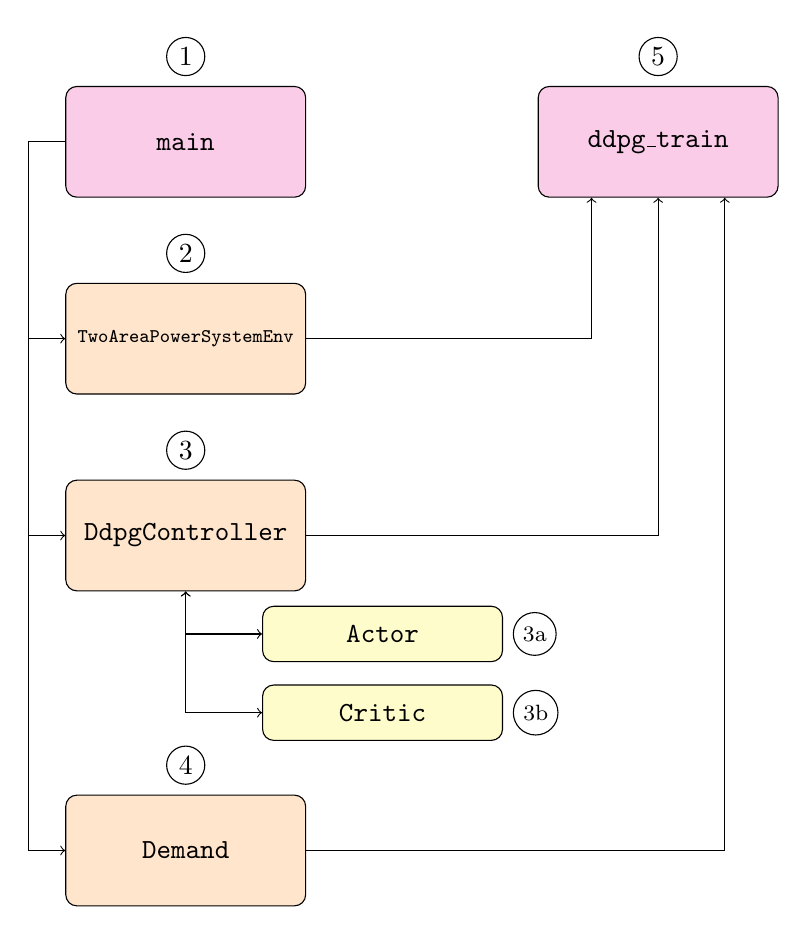
\begin{tikzpicture}[node distance = 2cm, auto]
    
    % Place script nodes
    \node [script, label=\circled{1}] (main) {\texttt{main}};
    \node [coordinate, left of=main] (p1) {};
    \node [script, right of=main, label=\circled{5}] (ddpg) {\texttt{ddpg\_train}};
  	
  	% Place class nodes
    \node [class, below of=main, label=\circled{2}] (env) {\scriptsize \texttt{TwoAreaPowerSystemEnv}};
    \node [class, below of=env, label=\circled{3}] (agent) {\texttt{DdpgController}};
    \node [coordinate, right of=agent, node distance=2.5cm] (p2) {};
    \node [class, below of=agent, node distance=4cm, label=\circled{4}] (demand) {\texttt{Demand}};
    
    % Place subclass node
    \node [subclass, below of=p2, node distance=1.25cm, label=0:\circled{\footnotesize 3a}] (actor) {\texttt{Actor}};
    \node [subclass, below of=actor, node distance=1cm, label=0:\circled{\footnotesize 3b}] (critic) {\texttt{Critic}};
    
    % Draw edges to classes
    \draw (main) -- (p1);
    \draw [->] (p1) |- (env);
    \draw [->] (p1) |- (agent);
    \draw [->] (p1) |- (demand);
    
    % Draw edge to subclass
    \draw[<->] (agent) |- (actor);
    \draw[<->] (agent) |- (critic);
    
    % Draw edge to training function
    \draw [->] (env) -| (ddpg.220);
    \draw [->] (agent) -| (ddpg);
    \draw [->] (demand) -| (ddpg.320);
    
\end{tikzpicture}

\end{document}